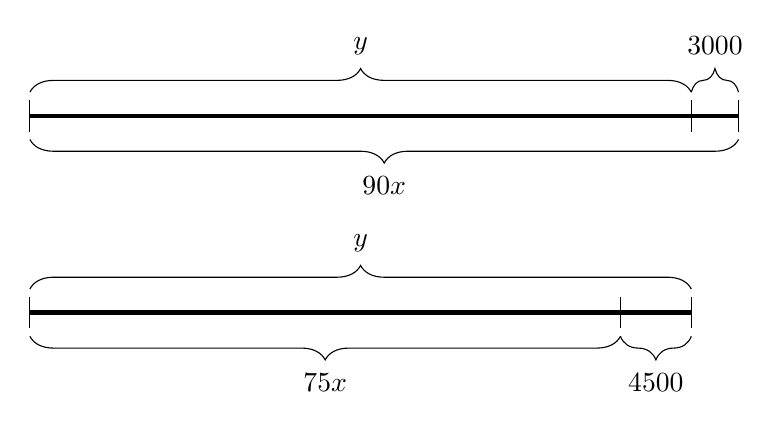
\begin{tikzpicture}
    \begin{scope}
        \pgfmathsetmacro{\a}{0}
        \pgfmathsetmacro{\b}{4.2*2}
        \pgfmathsetmacro{\c}{4.5*2}

        \draw [ultra thick] (\a, 0) -- (\c, 0);
        \foreach \x in {\a, \b, \c} {
            \draw (\x, 0.2) -- (\x, -0.2);
        }
        \draw[decorate, decoration={brace, amplitude=0.3cm}] (\a, 0.3) -- (\b, 0.3)
            node [pos=0.5, above=1em, align=center] {$y$};
        \draw[decorate, decoration={brace, amplitude=0.3cm}] (\b, 0.3) -- (\c, 0.3)
            node [pos=0.5, above=1em, align=center] {$3000$};
        \draw[decorate, decoration={brace,mirror, amplitude=0.3cm}] (\a, -0.3) -- (\c, -0.3)
            node [pos=0.5, below=1em, align=center] {$90x$};
    \end{scope}

    \begin{scope}[yshift=-2.5cm]
        \pgfmathsetmacro{\a}{0}
        \pgfmathsetmacro{\b}{3.75*2}
        \pgfmathsetmacro{\c}{4.2*2}

        \draw [ultra thick] (\a, 0) -- (\c, 0);
        \foreach \x in {\a, \b, \c} {
            \draw (\x, 0.2) -- (\x, -0.2);
        }
        \draw[decorate, decoration={brace, amplitude=0.3cm}] (\a, 0.3) -- (\c, 0.3)
            node [pos=0.5, above=1em, align=center] {$y$};
        \draw[decorate, decoration={brace,mirror, amplitude=0.3cm}] (\a, -0.3) -- (\b, -0.3)
            node [pos=0.5, below=1em, align=center] {$75x$};
        \draw[decorate, decoration={brace,mirror, amplitude=0.3cm}] (\b, -0.3) -- (\c, -0.3)
            node [pos=0.5, below=1em, align=center] {$4500$};
    \end{scope}
\end{tikzpicture}
